% Standalone conceptual figure: the extrinsic cooperation ceiling, in pictures.
% Style follows rsc/traitors/tex/panel_diagram.tex. Not \input by main.tex.
% Intended to sit beside the Extrinsic Ceiling theorem (Section 3.3).
% Build: pdflatex main.tex
\documentclass[border=4pt]{standalone}
\usepackage{tikz}
\usepackage{amsmath}
\usetikzlibrary{arrows.meta, calc, positioning, decorations.pathreplacing}

\definecolor{coop}{HTML}{009E73}
\definecolor{defect}{HTML}{D55E00}
\definecolor{neutral}{HTML}{8C8C8C}
\definecolor{accent}{HTML}{0072B2}
\definecolor{warn}{HTML}{E69F00}

\begin{document}
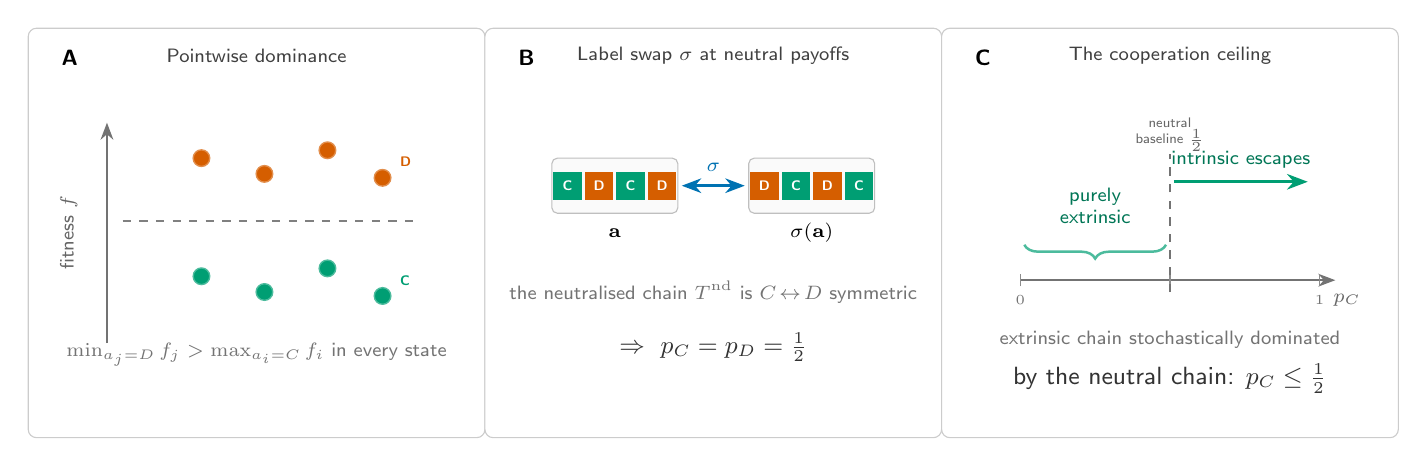
\begin{tikzpicture}[
    >=Stealth,
    font=\sffamily,
    sq/.style={rectangle, minimum size=0.36cm, inner sep=0pt, line width=0.5pt,
               font=\sffamily\tiny\bfseries, text=white},
    dot/.style={circle, minimum size=6pt, inner sep=0pt, line width=0.5pt},
    panellabel/.style={font=\sffamily\footnotesize\bfseries, anchor=north west},
    ptitle/.style={font=\sffamily\scriptsize, text=black!75, align=center},
    note/.style={font=\sffamily\scriptsize, text=black!55, align=center},
]

\def\pw{5.2}
\def\ph{4.6}
\def\gap{0.6}

\coordinate (P1) at (0, 0);
\coordinate (P2) at (\pw+\gap, 0);
\coordinate (P3) at (2*\pw+2*\gap, 0);

% Panel A: pointwise dominance (the hypothesis)
\begin{scope}[shift=(P1)]
    \draw[draw=black!20, fill=white, rounded corners=3pt]
        (-0.3,-0.3) rectangle (\pw+0.3, \ph+0.3);
    \node[panellabel] at (0, \ph+0.15) {A};
    \node[ptitle] at (\pw/2, \ph-0.05) {Pointwise dominance};

    % fitness axis
    \draw[->, black!55, line width=0.7pt] (0.7,0.9) -- (0.7,3.7);
    \node[font=\sffamily\scriptsize, text=black!60, anchor=south, rotate=90]
        at (0.45,2.3) {fitness $f$};

    % defectors high
    \foreach \x/\y in {1.9/3.25, 2.7/3.05, 3.5/3.35, 4.2/3.0} {
        \node[dot, fill=defect, draw=defect!70] at (\x,\y) {};
    }
    \node[font=\sffamily\tiny\bfseries, text=defect, anchor=west] at (4.3,3.2) {D};

    % separating line
    \draw[dashed, black!50, line width=0.6pt] (0.9,2.45) -- (4.6,2.45);

    % cooperators low
    \foreach \x/\y in {1.9/1.75, 2.7/1.55, 3.5/1.85, 4.2/1.5} {
        \node[dot, fill=coop, draw=coop!70] at (\x,\y) {};
    }
    \node[font=\sffamily\tiny\bfseries, text=coop, anchor=west] at (4.3,1.7) {C};

    \node[note] at (\pw/2, 0.75)
        {$\min_{a_j=D} f_j > \max_{a_i=C} f_i$ in every state};
\end{scope}

% Panel B: the label-swap symmetry sigma
\begin{scope}[shift=(P2)]
    \draw[draw=black!20, fill=white, rounded corners=3pt]
        (-0.3,-0.3) rectangle (\pw+0.3, \ph+0.3);
    \node[panellabel] at (0, \ph+0.15) {B};
    \node[ptitle] at (\pw/2, \ph-0.05) {Label swap $\sigma$ at neutral payoffs};

    % state a
    \draw[rounded corners=2pt, draw=black!25, fill=black!2]
        (0.55,2.55) rectangle (2.15,3.25);
    \foreach \k/\col/\lab in {1/coop/C,2/defect/D,3/coop/C,4/defect/D} {
        \pgfmathsetmacro{\x}{0.75 + (\k-1)*0.4}
        \node[sq, fill=\col] at (\x,2.90) {\lab};
    }
    \node[font=\sffamily\scriptsize] at (1.35,2.30) {$\mathbf{a}$};

    % sigma image
    \draw[rounded corners=2pt, draw=black!25, fill=black!2]
        (3.05,2.55) rectangle (4.65,3.25);
    \foreach \k/\col/\lab in {1/defect/D,2/coop/C,3/defect/D,4/coop/C} {
        \pgfmathsetmacro{\x}{3.25 + (\k-1)*0.4}
        \node[sq, fill=\col] at (\x,2.90) {\lab};
    }
    \node[font=\sffamily\scriptsize] at (3.85,2.30) {$\sigma(\mathbf{a})$};

    \draw[<->, accent, line width=0.9pt] (2.2,2.90) -- (3.0,2.90);
    \node[font=\sffamily\scriptsize, text=accent, anchor=south] at (2.6,2.95) {$\sigma$};

    \node[note] at (\pw/2, 1.55)
        {the neutralised chain $T^{\mathrm{nd}}$ is $C\!\leftrightarrow\!D$ symmetric};
    \node[font=\sffamily\small, text=black!80] at (\pw/2, 0.85)
        {$\Rightarrow\ p_C = p_D = \tfrac{1}{2}$};
\end{scope}

% Panel C: the ceiling
\begin{scope}[shift=(P3)]
    \draw[draw=black!20, fill=white, rounded corners=3pt]
        (-0.3,-0.3) rectangle (\pw+0.3, \ph+0.3);
    \node[panellabel] at (0, \ph+0.15) {C};
    \node[ptitle] at (\pw/2, \ph-0.05) {The cooperation ceiling};

    % p_C axis from x=0.7 (p=0) to x=4.5 (p=1); p=1/2 at x=2.6
    \draw[->, black!55, line width=0.7pt] (0.7,1.7) -- (4.7,1.7);
    \node[font=\sffamily\scriptsize, text=black!60, anchor=west] at (4.55,1.45) {$p_C$};
    \foreach \px/\lab in {0.7/0, 2.6/{\tfrac12}, 4.5/1} {
        \draw[black!45] (\px,1.62) -- (\px,1.78);
    }
    \node[font=\sffamily\tiny, text=black!55] at (0.7,1.45) {$0$};
    \node[font=\sffamily\tiny, text=black!55] at (4.5,1.45) {$1$};

    % baseline 1/2
    \draw[dashed, black!55, line width=0.7pt] (2.6,1.55) -- (2.6,3.3);
    \node[font=\sffamily\tiny, text=black!60, align=center] at (2.6,3.55)
        {neutral\\baseline $\tfrac12$};

    % extrinsic region [0,1/2]
    \draw[coop!70, line width=0.9pt, decorate,
          decoration={brace, amplitude=5pt, mirror}] (0.75,2.15) -- (2.55,2.15);
    \node[font=\sffamily\scriptsize, text=coop!75!black, align=center]
        at (1.65,2.65) {purely\\extrinsic};

    % intrinsic escape arrow above
    \draw[->, coop, line width=1.0pt] (2.65,2.95) -- (4.35,2.95);
    \node[font=\sffamily\scriptsize, text=coop!75!black, anchor=south]
        at (3.5,3.0) {intrinsic escapes};

    \node[note] at (\pw/2, 0.95)
        {extrinsic chain stochastically dominated};
    \node[font=\sffamily\small, text=black!80] at (\pw/2, 0.45)
        {by the neutral chain: $p_C \le \tfrac12$};
\end{scope}

\end{tikzpicture}
\end{document}
